\begin{figure}[H]
  \centering
  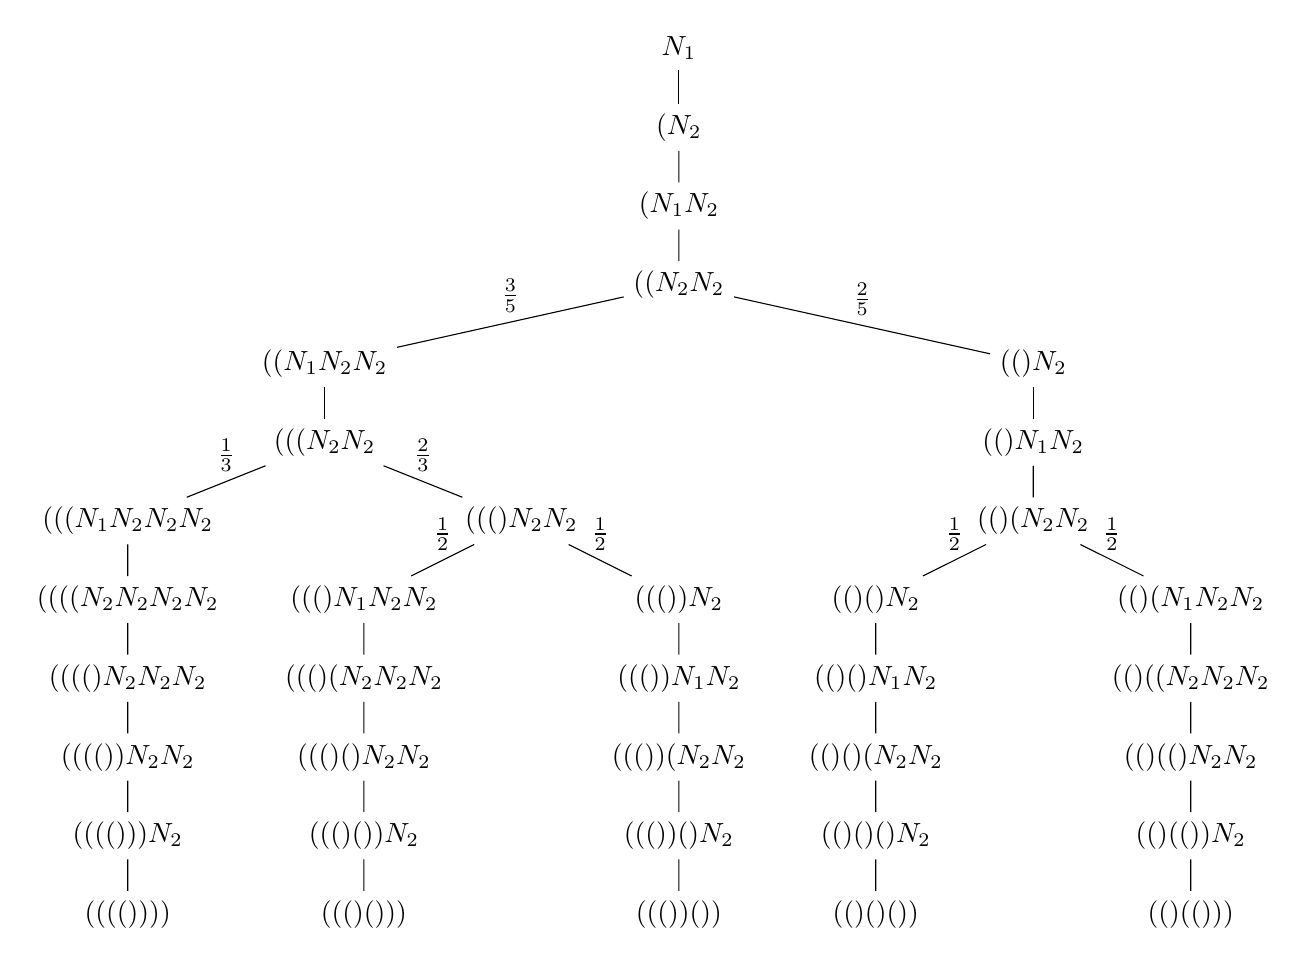
\begin{tikzpicture}[
    level distance=1cm,
    level 4/.style={sibling distance=9cm},
    level 6/.style={sibling distance=5cm},
    level 7/.style={sibling distance=4cm}]

  \node[] {$N_1$}
    child {node {$(N_2$}
      child {node {$(N_1N_2$}
        child {node {$((N_2N_2$}
          child {node {$((N_1N_2N_2$}
            child {node {$(((N_2N_2$}
              child {node {$(((N_1N_2N_2N_2$}
                child {node {$((((N_2N_2N_2N_2$}
                  child {node {$(((()N_2N_2N_2$}
                    child {node {$(((())N_2N_2$}
                      child {node {$(((()))N_2$}
                        child {node {$(((())))$}}
                      }
                    }
                  }
                }
                edge from parent         
                  node[above] {$\frac{1}{3}$}
              }
              child {node {$((()N_2N_2$}
                child {node {$((()N_1N_2N_2$}
                  child {node {$((()(N_2N_2N_2$}
                    child {node {$((()()N_2N_2$}
                      child {node {$((()())N_2$}
                        child {node {$((()()))$}}
                      }
                    }
                  }
                  edge from parent         
                    node[above] {$\frac{1}{2}$}
                }
                child {node {$((())N_2$}
                  child {node {$((())N_1N_2$}
                    child {node {$((())(N_2N_2$}
                      child {node {$((())()N_2$}
                        child {node {$((())())$}}
                      }
                    }
                  }
                  edge from parent         
                    node[above] {$\frac{1}{2}$}
                }
                edge from parent         
                  node[above] {$\frac{2}{3}$}
              }
            }
            edge from parent         
              node[above] {$\frac{3}{5}$}
          }
          child {node {$(()N_2$}
            child {node {$(()N_1N_2$}
              child {node {$(()(N_2N_2$}
                child {node {$(()()N_2$}
                  child {node {$(()()N_1N_2$}
                    child {node {$(()()(N_2N_2$}
                      child {node {$(()()()N_2$}
                        child {node {$(()()())$}}
                      }
                    }
                  }
                  edge from parent         
                    node[above] {$\frac{1}{2}$}
                }
                child {node {$(()(N_1N_2N_2$}
                  child {node {$(()((N_2N_2N_2$}
                    child {node {$(()(()N_2N_2$}
                      child {node {$(()(())N_2$}
                        child {node {$(()(()))$}}
                      }
                    }
                  }
                  edge from parent         
                    node[above] {$\frac{1}{2}$}
                }
              }
            }
            edge from parent         
              node[above] {$\frac{2}{5}$}
          }
        }
      }
    };
    
  \end{tikzpicture}
  \caption{Derivations tree with probabilties of strings of length 8}
\end{figure}